
% !Mode:: "TeX:UTF-8" (encoding info for WinEdt)
\section{Privatnotizen}\label{Privatnotizen}
Einbindung vertraulicher Texte in den Konsultationseintrag. Dieses Plugin ist Teil der Standard-Distribution.


Manchmal müssen Anmerkungen in eine KG eingetragen werden, die nicht von anderen Praxismitarbeitern eingesehen werden sollen, und die auch nicht bei einem allfälligen Export der KG mit exportiert werden sollen (z.B. vertrauliche Informationen von Dritten).
Dieses Plugin ermöglicht solche \textit{Privatnotizen}: Wenn es installiert ist, erscheint bei Rechtsklick im Konsultationsfenster ein Menüpunkt \textit{Notiz}:

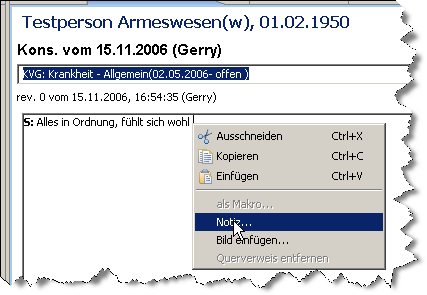
\includegraphics[width=3in]{images/notiz1.png}
% notiz1.png: 427x295 pixel, 96dpi, 11.30x7.80 cm, bb=0 0 320 221

Wenn Sie diesen Punkt anklicken, können Sie beliebigen Text eingeben:

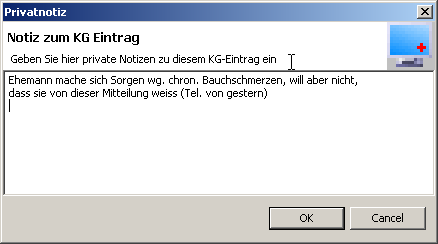
\includegraphics[width=3in]{images/notiz2.png}
% notiz2.png: 438x244 pixel, 96dpi, 11.59x6.46 cm, bb=0 0 328 183

Nach Klick auf \textit{OK} weist ein \textit{Notiz}-Querverweis auf diese Notiz hin:

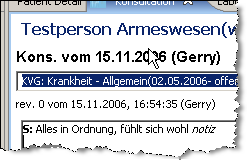
\includegraphics[width=3in]{images/notiz3.png}
% notiz3.png: 247x160 pixel, 96dpi, 6.53x4.23 cm, bb=0 0 185 120

Mit Anklicken dieses Querverweises wird jeweils das Fenster mit der Notiz wieder angezeigt. Wenn ein anderer Benutzer angemeldet ist, wird nichts angezeigt.

Bei einem Export oder Drucken der KG werden diese Notizen übergangen.


